\chapter{Data Loading and Comparison}
\section{Transforming Raw Data to structured format: Extract, Load, Transform}\label{sec:elt}
Raw data from the experiment is stored in \gls{HDF5} files. This includes many \gls{beamline} diagnostic information such as \gls{BAM}, \gls{GMD}, the delay stage readings, the monochromator energy, sample specific information such as extractor voltage, and the electron counting in the 3 detector dimensions corresponding to the \gls{DLD} spatial X and Y axes and the temporal time axis. This information is resolved at each bunch of electrons coming from the accelerator called a \gls{train}, which are further microbunched into \glsplural{pulse}.

The \gls{OpenCOMPES} was established to develop tools and infrastructure to make analysis easier. To this end, a modular Python library called \texttt{\gls{SED}} was created that provides the entire pipeline from easy data loading to common calibration and corrections, multidimensional binning to create images, and saving the images to standard formats, with proper care of data provenance.

The data pipeline follows an \gls{ELT} process, wherein raw data is extracted from \gls{HDF5} files, transformed into a structured format suitable for analysis, and subsequently stored in intermediate buffer files for further downstream processes such as analysis and visualization.

The following sections provide a detailed exposition of each stage of this \gls{ELT} process, also shown in \cref{fig:elt}. The first stage, extraction, begins with the loading of raw data from the \gls{HDF5} files. These files encapsulate experimental results across multiple channels, including electron-resolved and time-resolved data. The hierarchical structure of the \gls{HDF5} files allows the organization of data into groups, where each group contains an index and its corresponding dataset, collectively referred to as a “channel” The paths to these \gls{HDF5} files, along with relevant configuration parameters, are provided to the pipeline to dictate the steps of the subsequent transformation process.

\section*{Pipeline Overview}
To optimize performance and facilitate data management, the pipeline generates buffer files for each type of data (electron and time-resolved). This task is handled by the \texttt{BufferFilePaths} class, which initializes file paths and manages the creation of buffer files in the efficient \texttt{Parquet} format. By checking the presence of pre-existing buffer files, the class determines whether to reuse these files or regenerate them, based on the \texttt{force\_recreate} flag.

Each \gls{HDF5} file results in the generation of two primary buffer files: one containing electron-resolved data and another containing pulse/train-resolved data. These files are essential for organizing the data at the pulse level and maintaining resolution at the electron level. The data for each train contains roughly 500 pulses, and although some data is resolved at the pulse level, each index often holds an array, necessitating the use of the \texttt{pandas} MultiIndex functionality to maintain the data’s hierarchical structure. Detector measurements, which are electron-resolved along the X, Y, and temporal axes, are typically represented as three-dimensional arrays and add further complexity to the indexing process.

A critical transformation step involves correcting for offsets in pulse IDs to ensure accurate synchronization of data across different channels. Any data associated with pulse IDs below zero is removed, as it is considered invalid. Similarly, \texttt{NaN} pulses are dropped to avoid introducing inconsistencies in downstream analyses. While it is possible that pulses exceeding 500 may also be invalid, these are not filtered during this stage, as that determination is deferred to the final analysis. Due to machine fluctuations, pulses may become unsorted, and hence the pulses are sorted within each train to maintain temporal order.

Once this cleaning process is completed, electron-resolved channels are combined using an outer join with pulse and train-resolved channels, forming a comprehensive dataframe that contains all relevant information for further analysis. This merged dataset is separated into two primary dataframes: the electron-resolved dataframe and the pulse-resolved dataframe.

The electron dataframe contains only rows where electron events have been detected, with any missing data in non-electron channels forward-filled to ensure completeness. This dataframe serves as the main source of electron-specific data for further analyses. However, given that not all pulses or trains may produce electron events, a separate pulse-resolved dataframe is generated to capture all available train and pulse data, independent of electron detections. This pulse-resolved dataframe is essential for normalization steps involving time-resolved channels, such as those related to the delay axis.

The pipeline also includes validation steps for auxiliary channels, particularly those containing multidimensional data (e.g., 4D arrays), ensuring that all required channels exist within the files before proceeding with further transformations.

After this initial transformation and extraction, the buffer files are saved in \texttt{Parquet} format, chosen for its efficiency in storage and speed of access during future computations. The final stage involves the loading of all these buffer files into a unified dataframe using \texttt{Dask}, a distributed computing library that enables scalable processing of large datasets. At this stage, forward-filling is again applied to non-electron channels, ensuring that missing values between files are handled consistently. However, care must be taken when forward-filling across different runs, as this could introduce inter-run inconsistencies.

Finally, the schema of the buffer files is cross-validated against the predefined list of channels to ensure consistency and completeness prior to loading the data into \texttt{Dask}.

\begin{figure}[H]
    \label{fig:elt}
    \centering
    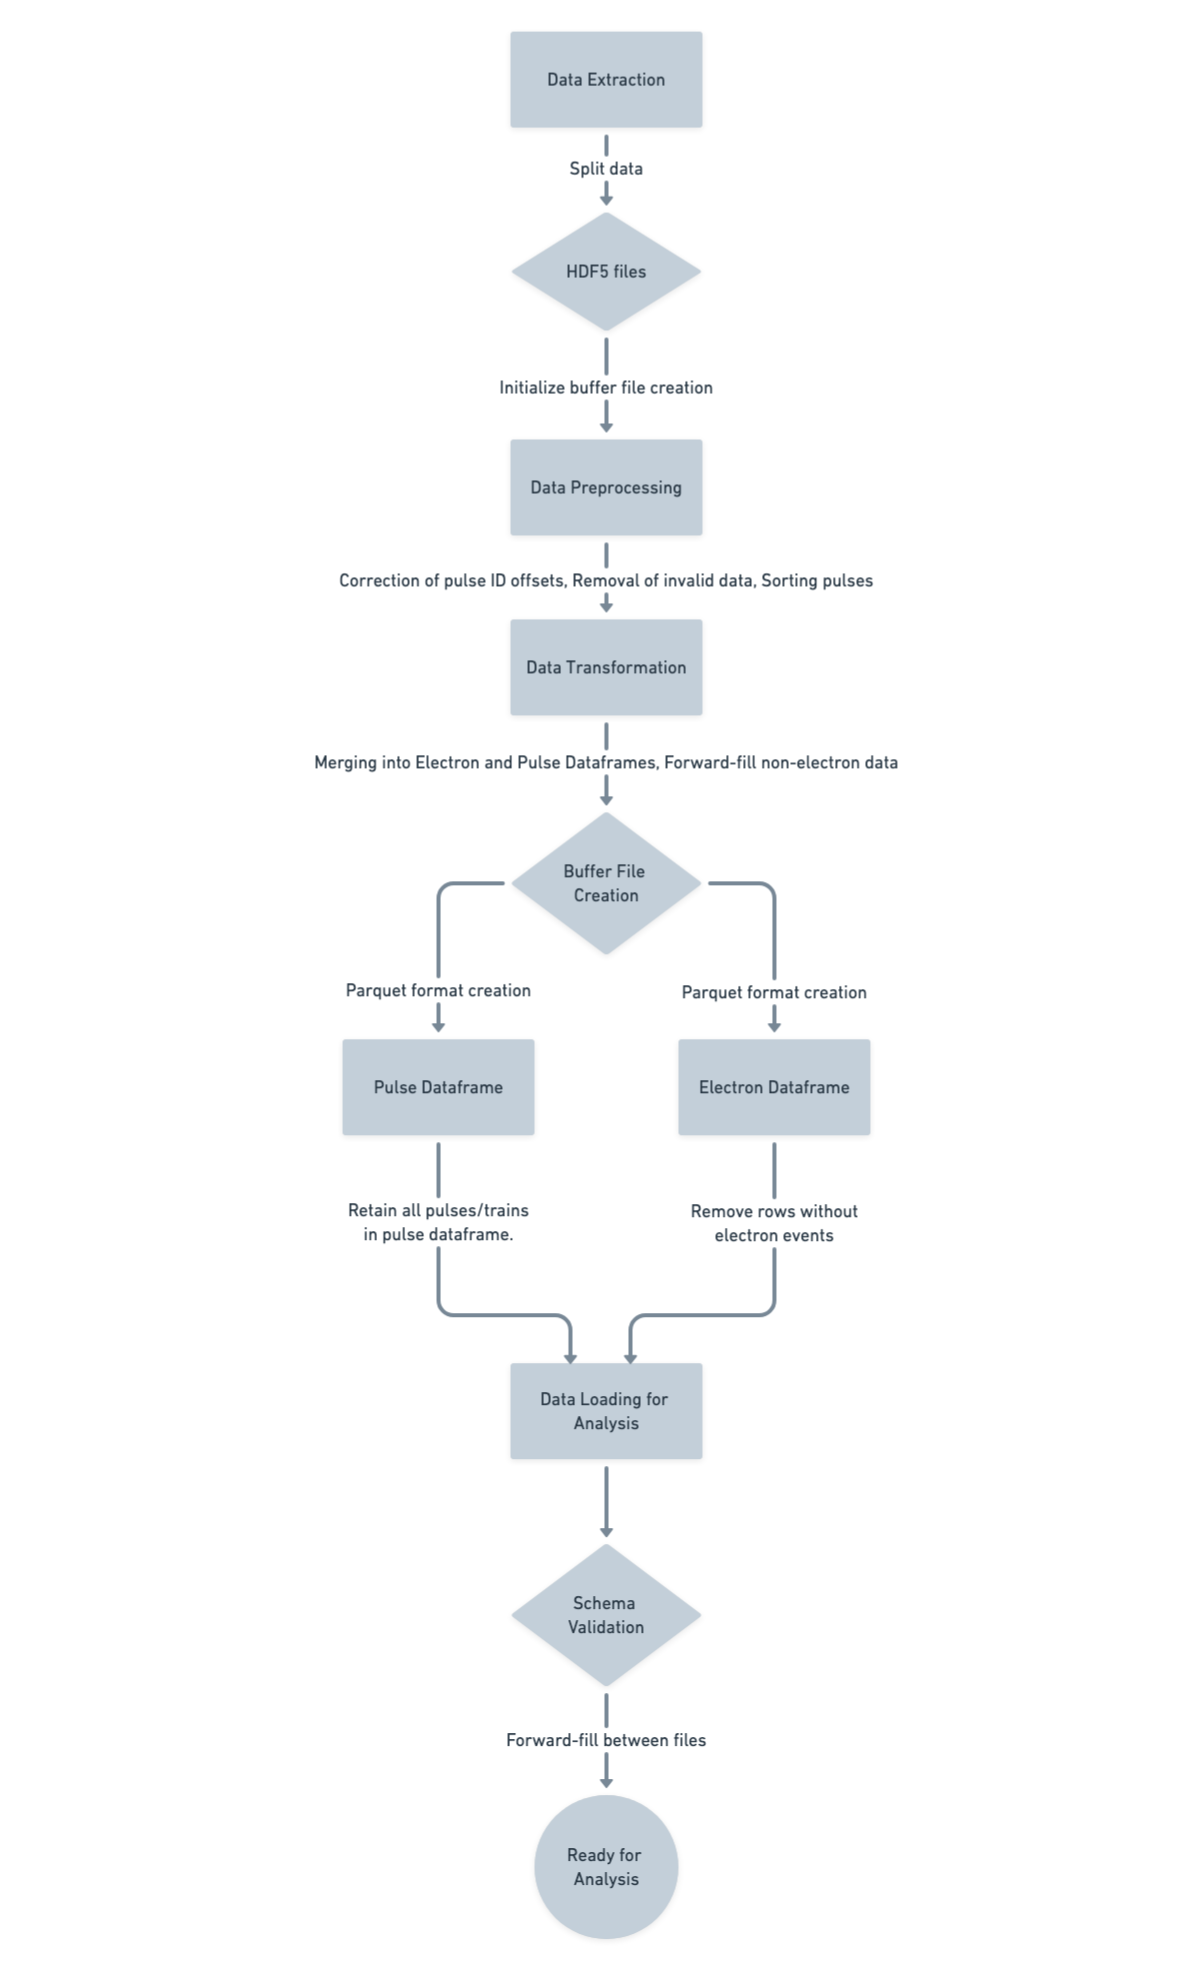
\includegraphics[width=0.7\linewidth]{images/elt_cropped.png}
    \caption{Complete \gls{ELT} pipeline for the data from \gls{HEXTOF} at \gls{FLASH}}
\end{figure}

\section{Metrics}

\Gls{MSE} is a common measure of the average squared differences between predicted values and actual values. It quantifies the error in a model’s predictions, where lower values indicate better performance. It is sensitive to outliers since squaring the differences amplifies larger errors.

\begin{note}
    {\Glsxtrfull{MSE}}
    \begin{equation}
        \text{MSE} = \frac{1}{N} \sum_{i=1}^{N} (x_i - y_i)^2
    \end{equation}
    \begin{itemize}
        \item $x_i$: pixel value of the noisy image
        \item $y_i$: pixel value of the target image
        \item $N$: total number of pixels
    \end{itemize}
\end{note}

\Gls{PSNR} is a measure of the peak error between two images, often used to evaluate image compression quality. It expresses the ratio between the maximum possible power of a signal and the power of corrupting noise. Higher PSNR values indicate better quality.

\begin{note}
    {\Glsxtrfull{PSNR}}
    \begin{equation}    
        \text{PSNR} = 10 \log_{10} \left( \frac{L^2}{\text{MSE}} \right)
    \end{equation}
    \begin{itemize}
        \item $L$: maximum pixel value of the image
        \item \gls{MSE}: mean squared error
    \end{itemize}
\end{note}


\Gls{SSIM} is a perceptual metric that quantifies the visual impact of three characteristics of an image: luminance, contrast, and structure. It evaluates the similarity between two images based on their structural information, making it more aligned with human visual perception than MSE or PSNR. Values range from -1 to 1, with 1 indicating perfect similarity.
\begin{note}
    {\Glsxtrfull{SSIM}}
    \begin{equation}    
        \text{SSIM}(x, y) = \frac{(2\mu_x \mu_y + C_1)(2\sigma_{xy} + C_2)}{(\mu_x^2 + \mu_y^2 + C_1)(\sigma_x^2 + \sigma_y^2 + C_2)}
    \end{equation}
    \begin{itemize}
        \item $\mu_x, \mu_y$: mean of $x$ and $y$
        \item $\sigma_x, \sigma_y$: standard deviation of $x$ and $y$
        \item $\sigma_{xy}$: covariance of $x$ and $y$
        \item $C_1 = (k_1L)^2, C_2 = (k_2L)^2$: constants to stabilize the division
    \end{itemize}
\end{note}

\Gls{MSSSIM} extends \gls{SSIM} by evaluating image similarity across multiple scales and resolutions. By considering different image scales, it captures more information about structural variations and perceptual quality, making it particularly useful for assessing image quality in applications like compression. Similar to \gls{SSIM}, higher values indicate greater similarity.

\begin{note}
    {\Glsxtrfull{MSSSIM}}
    \begin{equation}    
        \text{MSSSIM}(x, y) = \prod_{j=1}^{J} \text{SSIM}(x_j, y_j)^{\alpha_j}
    \end{equation}
    \begin{itemize}
        \item $J$: number of scales
        \item $x_j, y_j$: images at scale $j$
        \item $\alpha_j$: weight for scale $j$, summing to 1
    \end{itemize}
\end{note}


\section{Experiment: Metric Comparison}\label{sec:metric_comparison_experiment}

The objective of this experiment is to evaluate the effectiveness of various image quality metrics (\gls{MSE}, \gls{PSNR}, \gls{SSIM}, and \gls{MSSSIM}) when the provided reference is noisy. Specifically, reconstructed images from a trained neural network, that has shown clear improvements in perpetual quality, are compared against the high-count but noisy reference. Examples of such images at different counts can be seen in Figure~\ref{fig:images-noisy-denoised}, which shows how the noisy images are devoid of any features at low counts, while the denoised images show clear features similar to the target. For this analysis, it is not relevant if the high quality reconstructions are due to overfitting or not, but rather that they produce perpetually better quality images (sometimes even compared to the target). So the hope is that the metrics acknowledge this improvement.

\begin{figure}[h]
    \centering
    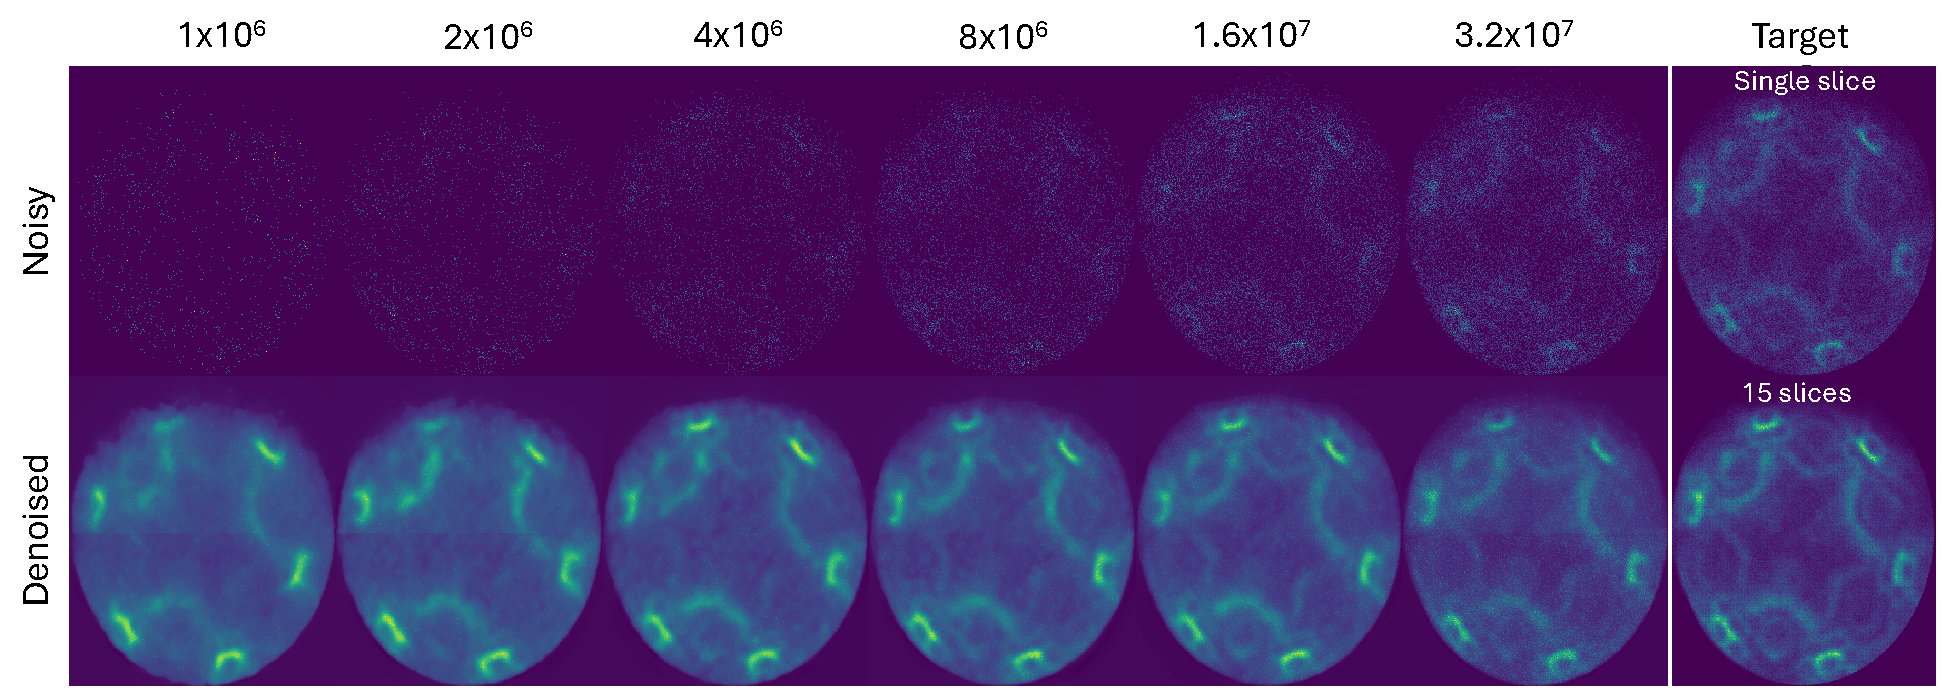
\includegraphics[width=1\linewidth]{images/images_noisy_denoised_with_target.pdf}
    \caption{The low-count noisy images and the perpetually better denoised images shown for different electron counts (in Millions) and the noisy target images (single slice and window-averaged 15 slices). Below \num{8}M counts, none of the features are discernable for noisy images, while the denoised images show clear features similar to the target.}
    \label{fig:images-noisy-denoised}
\end{figure}

The \gls{GrIr} dataset is used, with electron counts ranging from \numrange{1e6}{3.2e7}. For each total count, a set of 2D noisy images (referred to as noisy slices) is extracted from the dataset. Corresponding high-count 2D slices (referred to as target slices) are used as reference images for comparison (from the dataset with \num{1.86e8} counts). Likewise, reconstructed images from the neural network are also compared against the target slices.

\begin{table}[h]
    \centering
    \caption{Comparison Types and Metrics}
    \begin{tabular}{p{0.24\linewidth} | p{0.49\linewidth} | p{0.19\linewidth}}
        \hline
        \textbf{Comparison Type} & \textbf{Description} & \textbf{Metrics Evaluated} \\
        \hline
        Noisy & Input image is a noisy realization of target & MSE, PSNR, SSIM, MS-SSIM \\
        \hline
        Denoised & Input image is perpetually of better quality & MSE, PSNR, SSIM, MS-SSIM \\
        \hline
    \end{tabular}
    \caption{Comparison types and metrics evaluated in the experiment. This is repeated for single slice and window-averaged images.}
    \label{tab:comparison_types}
\end{table}

The metric evaluation procedure involves a data loader, implemented using the \texttt{PyTorch Dataset} class, which iterates through the different datasets and extracts noisy and target 2D image slices (window-averaged or single slice). For each pair of noisy and target slices, the metrics are computed. The comparison results are then grouped by acquisition count and type (noisy vs. denoised).

This metric comparison is performed with \texttt{1638} images sliced along each dimension of the dataset. The results are aggregated and a 95\% confidence interval is calculated for each metric to assess the reliability of the comparison. Table~\ref{tab:comparison_types} summarizes the comparison types and metrics evaluated in this experiment, repeated for both single slice and window-averaged images.


\begin{figure}[h]
    \centering
    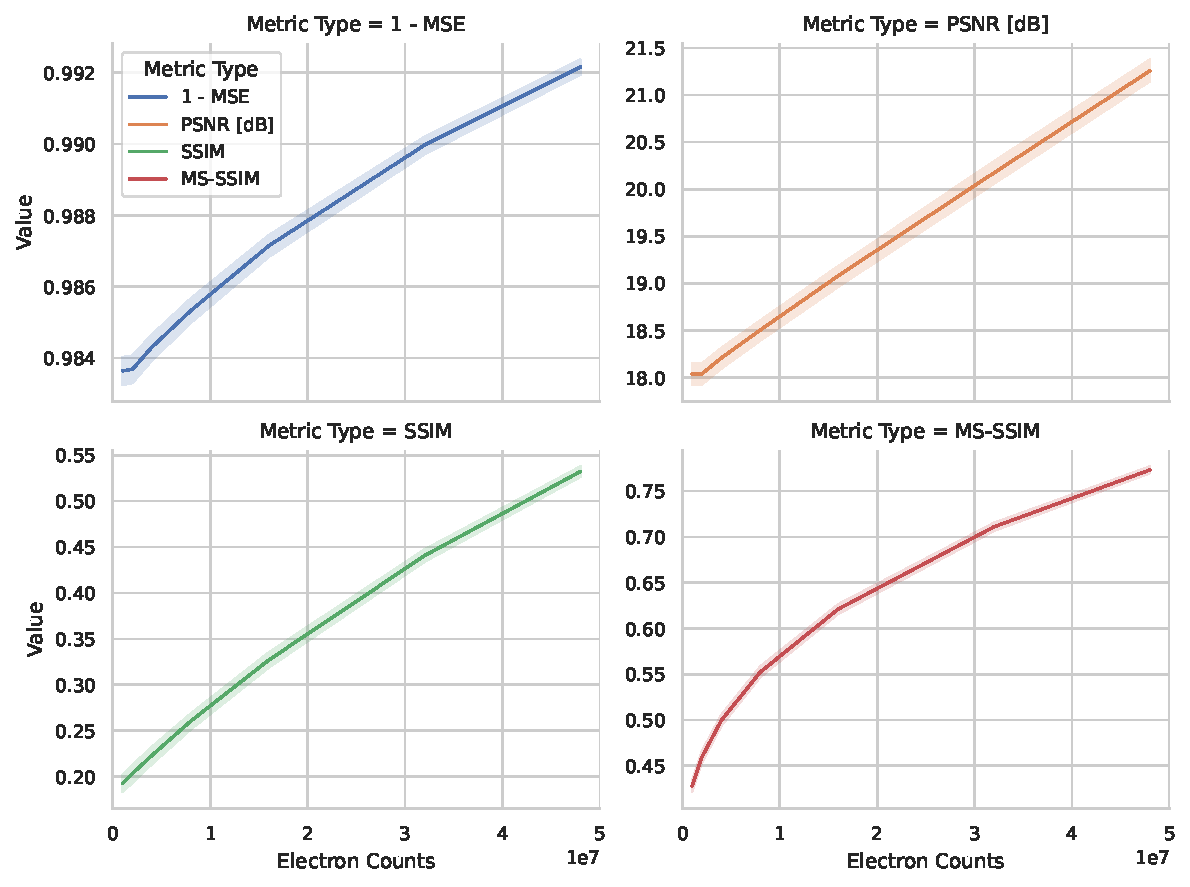
\includegraphics[width=1\linewidth]{images/metrics_comparison_same_target.pdf}
    \caption{Comparison of image quality metrics (\gls{MSE}, \gls{PSNR}, \gls{SSIM}, \gls{MSSSIM}) with noisy realization of a noisy target. The metrics show improved results with increased electron counts, as noise levels decrease. \gls{MSSSIM} shows the best relative improvement in metrics lower counts below \num{e7}.}
    \label{fig:metrics-comparison-noisy}
\end{figure}

Comparing the noisy images with target, all metrics trivially show an improvement with increased counts (less noise) (see Figure~\ref{fig:metrics-comparison-noisy}). However, \gls{MSE}, \gls{PSNR} and \gls{SSIM} show deteriorated metrics when comparing against perpetually high quality images (Figure~\ref{fig:metrics-comparison}). This can be attributed to the presence of noise in the reference image. For higher counts, \gls{SSIM} manages to show improved results, whereas \gls{MSE} report \gls{PSNR} consistently worse results compared to the noisy images. \gls{MSSSIM} consistently reports better results with the higher quality images, making it the most reliable metric for evaluation.

\begin{figure}
    \centering
    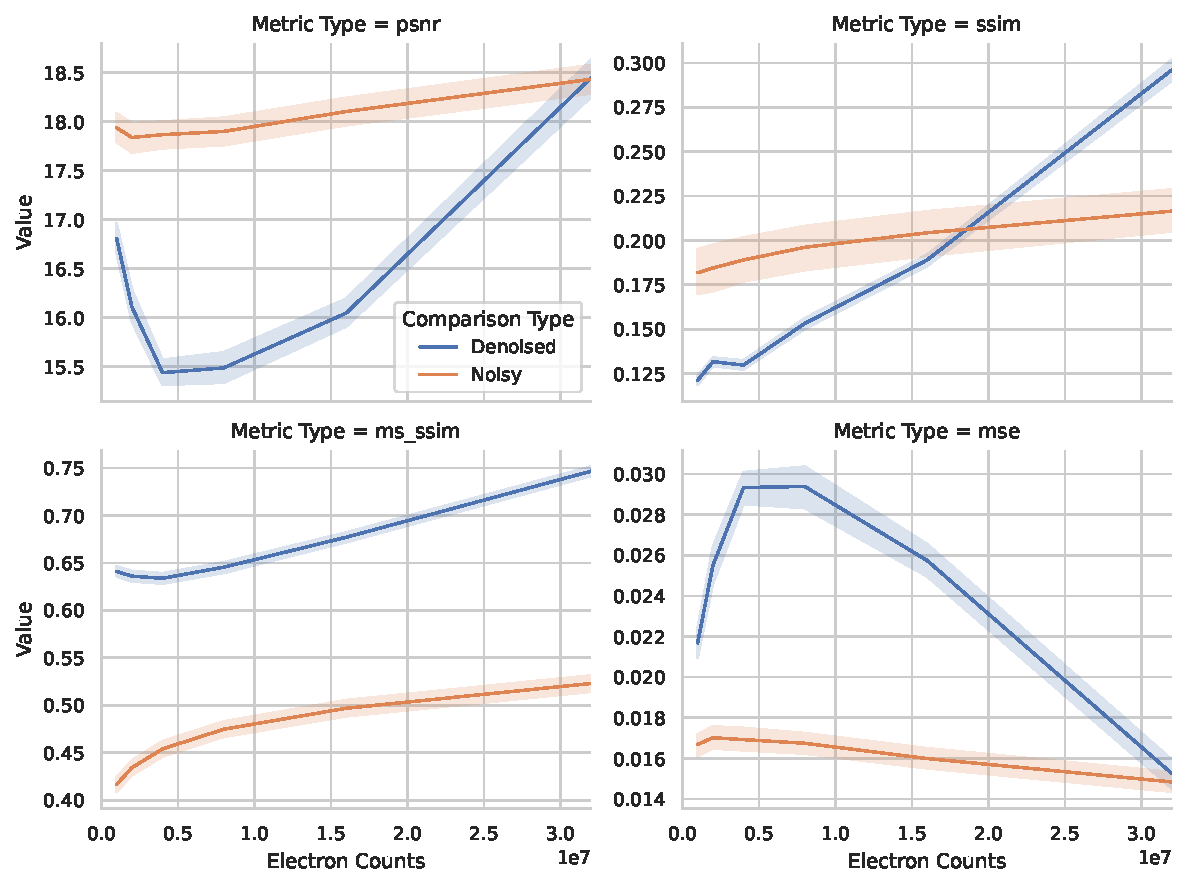
\includegraphics[width=1\linewidth]{images/metrics_comparison_denoised_noisy.pdf}
    \caption{Shows comparison of evaluating metrics (\gls{MSE}, \gls{PSNR}, \gls{SSIM}, \gls{MSSSIM}) with the input being a noisy realization of target or denoised version of that realization. Both are compared to a high-count target that is also noisy. Trivially, all metrics show an improvement when the counts increase. However, \gls{MSE} and \gls{PSNR} evaluate better when the input is noisy, while \gls{SSIM} and \gls{MSSSIM} show better results when the input is denoised. The gap between noisy and denoised is more pronounced for \gls{MSSSIM} than \gls{SSIM}, hence the better metric. }
   \label{fig:metrics-comparison}
\end{figure}

Additionally, we investigate the effect of window-averaged reference images on the metrics. Results indicate that the window-averaged references improve metric outcomes, as the gap between the metrics calculated with noisy and high quality images split up further. Consequently, we adopt the window-averaged images as reference for the denoising evaluation.


\begin{figure}
    \centering
    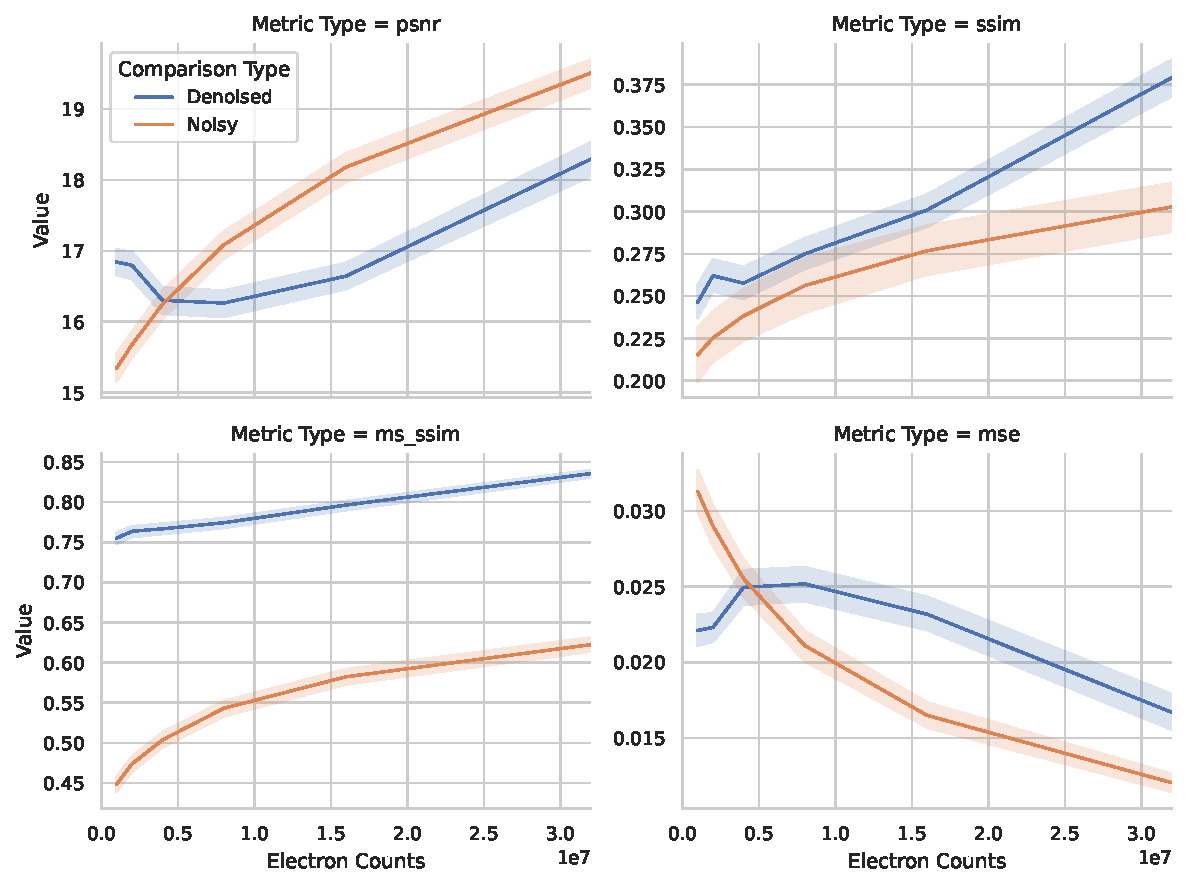
\includegraphics[width=1\linewidth]{images/metrics_comparison_denoised_noisy_averaged.pdf}
    \caption{Metrics comparison for noisy 2D slices against a window-averaged target slice. The window-averaged target does not significantly improve the reported metrics, showing that averaging over neighboring slices reduces resolution and does not offer a superior reference for denoising evaluation.}
    \label{fig:metrics-comparison-averaged-target}
\end{figure}